\documentclass{cis320}
\usepackage{listings}
\usepackage{xcolor}
\usepackage{lmodern}
\usepackage{listings}
\usepackage{physics}
\usepackage{graphicx}
\usepackage{subfig}

%New colors defined below
\definecolor{codegreen}{rgb}{0,0.6,0}
\definecolor{codegray}{rgb}{0.5,0.5,0.5}
\definecolor{codepurple}{rgb}{0.58,0,0.82}
\definecolor{backcolour}{rgb}{0.95,0.95,0.92}

%Code listing style named "mystyle"
\lstdefinestyle{mystyle}{
  backgroundcolor=\color{backcolour}, commentstyle=\color{codegreen},
  keywordstyle=\color{magenta},
  numberstyle=\tiny\color{codegray},
  stringstyle=\color{codepurple},
  basicstyle=\ttfamily\footnotesize,
  breakatwhitespace=false,         
  breaklines=true,                 
  numbers=none,             
  keepspaces=true,                                     
  numbersep=5pt,                  
  showspaces=false,
  language=[90]Fortran,                
  showstringspaces=false,
  showtabs=false,                  
  tabsize=2
}
\lstset{style=mystyle}
\addbibresource{./Sources.bib}

\begin{document}
\noindent Homework \textbf{LTTC Quantum dynamics}\hfill  Mauro Gascon Navas\\
TCCM \today

\hrulefill

\section{Spherical confinement potential}

A Spherical Confinement Potential (SCP) is added to as an option the program to ensure that the particles do not "escape" the simulation. The potential energy is defined as:
\[
E = 0.008 \cdot (dist_{com}-R_{max})^4 = 0.008 \cdot (\abs{\vec{r}}-R_{max})^4, \quad \abs{\vec{r}} > R_{max} 
\]
Where the center of mass (com) is defined as the origin. The force is then calculated as the gradient:
\[
\begin{aligned}
F = -\nabla E &= -\nabla \left( 0.008 \cdot (\abs{\vec{r}}-R_{max})^4 \right) \\
&= -4 \cdot 0.008 \cdot (\abs{\vec{r}}-R_{max})^3 \cdot \nabla \abs{\vec{r}} \\
&=-0.032 \cdot (\abs{\vec{r}}-R_{max})^3 \cdot \frac{\vec{r}}{\abs{\vec{r}}}
\end{aligned}
\]

The subroutine \textit{apply\_scp} is added to the program to calculate the forces and potential energy due to the SCP. The subroutine takes as inputs the number of atoms, the positions, forces, potential energy and the radius of the confinement. The center of mass is calculated and the forces are updated for each atom.\\
\par
At every step, the COM is calculated and all particles are translated so it is centered at the origin. then de distances are computed and the forces and potntial energies of for the particles that are outside the confinement are updated.\\
The subroutine is called at the end of the main loop, after the forces are calculated.\\
\par
A sample run for a system of 125 atoms (\textit{liquid-argon.xyz}) confined with $R_{max}=23$ \r{A} is  provided in Figure \ref{fig:SCP}. To check the conservation of energy, an NVE simmulation is performed setting the initial temperature to 0 K to avoid random conditions (see Section 2). All the kinetic energy of the system comes from the energy stored in the non-optimal initial geometry. As we can see, the total energy remains constant through the simmulation, and its small noise can be explained from the timestep (which needs to be large to actually generate geometries where the SCP is activated) and the very steep r dependence ($SCP \sim r^4$) of the potential. \\
The command to run it in this implementation is:

\begin{lstlisting}[language=bash]
  ./md_program -FILE liquid-argon.xyz -SAVEFREQ 100 -TIMESTEP 1 -MAX_MD_STEPS 100000  -SCP 23 -TEMP 0\end{lstlisting}

\begin{figure}[th!]
    \centering
    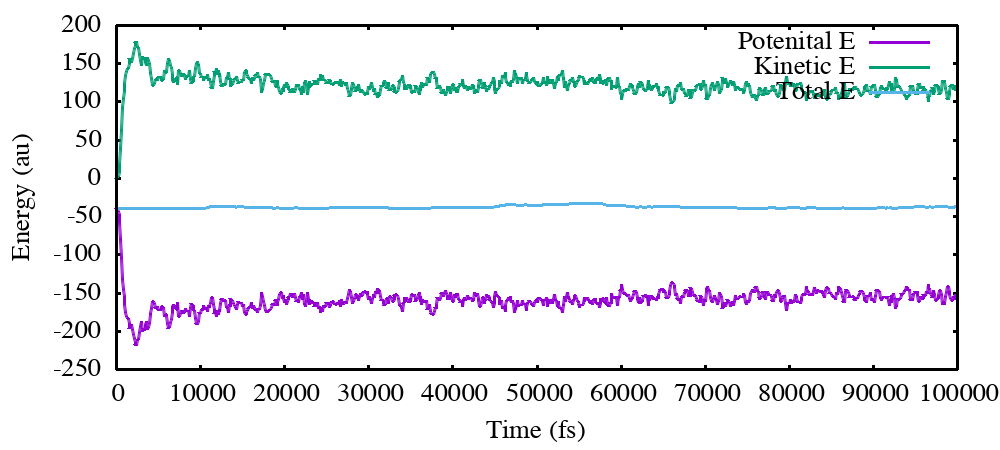
\includegraphics[width=0.8\textwidth]{SCP.png}
    \caption{NVE simmulation of 125 Ar atoms in a SCP with $R_{max}=23$ \r{A}}
    \label{fig:SCP}
\end{figure}

\begin{lstlisting}[caption=Subroutine to apply a SCP.]
subroutine apply_scp(forces,pot_ener,positions,nbr_atomes,R_scp)
    implicit none
    
    integer,intent(in)                                    :: nbr_atomes
    real*8, intent(in)                                    :: R_scp
    real*8, allocatable, dimension (:,:),intent(inout)       :: positions
    real*8, allocatable, dimension (:,:),intent(inout)    :: forces
    real*8,intent(inout)                                  :: pot_ener
    real*8, dimension(3)  :: com
    real*8  :: d_com
    integer :: i,j
    
    com = 0.0d0 ! Get center of Mass
    do i=1,nbr_atomes
        do j=1,3
        com(j)=com(j)+positions(i,j) !if we had diffrent masses we would have to "mass-avarage"
        enddo
    enddo
    com=com/dble(nbr_atomes) 
    
    do i=1,nbr_atomes !!Apply SCP
        d_com = 0.0d0
        do j=1,3
        positions(i,j) = positions(i,j) - com(j) ! Center the system
        d_com = d_com + positions(i,j)**2 ! Distance to origin (COM)
        enddo
        d_com = sqrt(d_com)-R_scp
        if (d_com .gt. 0.0d0) then
        pot_ener = pot_ener + 0.008d0*(d_com)**4 ! update potential energy
        do j=1,3
            forces(i,j) = forces(i,j) -0.032*(d_com)**3*positions(i,j)/(d_com+R_scp) !update forces calculateed previously
        enddo
        end if
    enddo
end subroutine apply_SCP \end{lstlisting}

\section{Initial random velocities}
To genereate the initial velocities following the boltzman distribution utilizing the given subroutine \textit{gaussian\_distr} to generate random numbers with a normal distribution. The subroutine \textit{initial\_velocities} is added to the program to initialize the velocities of the particles. The subroutine takes as inputs the number of atoms, the velocities, the temperature and the mass of the particles. The velocities are updated for each atom.\\
\par
In Figure \ref{fig:dist} the results of $10^{-6}$ points of \textit{initial\_velocities} and \textit{gaussian\_distr()} are compared to their expectation, showing its correct functioning.\\

\begin{figure}[h]
    \centering
    \subfloat[\textit{gauss\_distr()}]{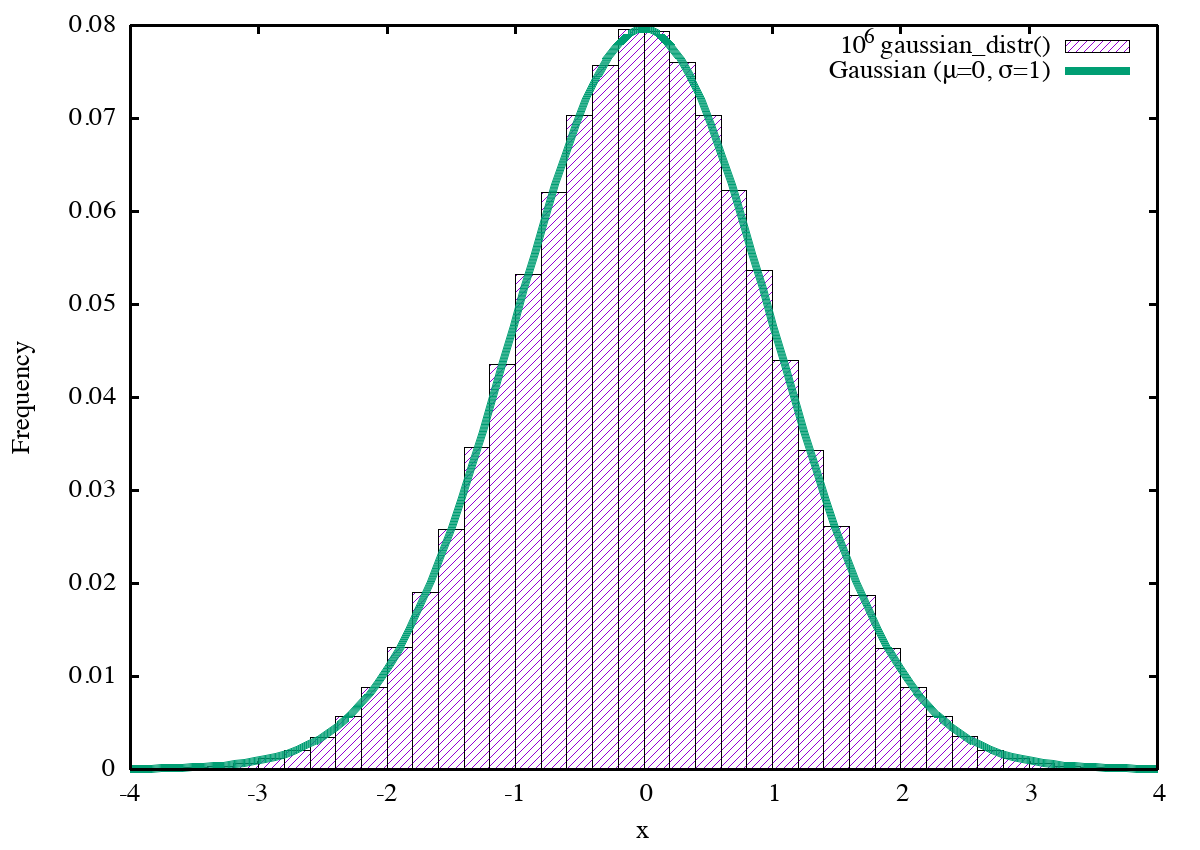
\includegraphics[width=0.5\textwidth]{Gauss.png}}
    \subfloat[\textit{initial\_velocities}]{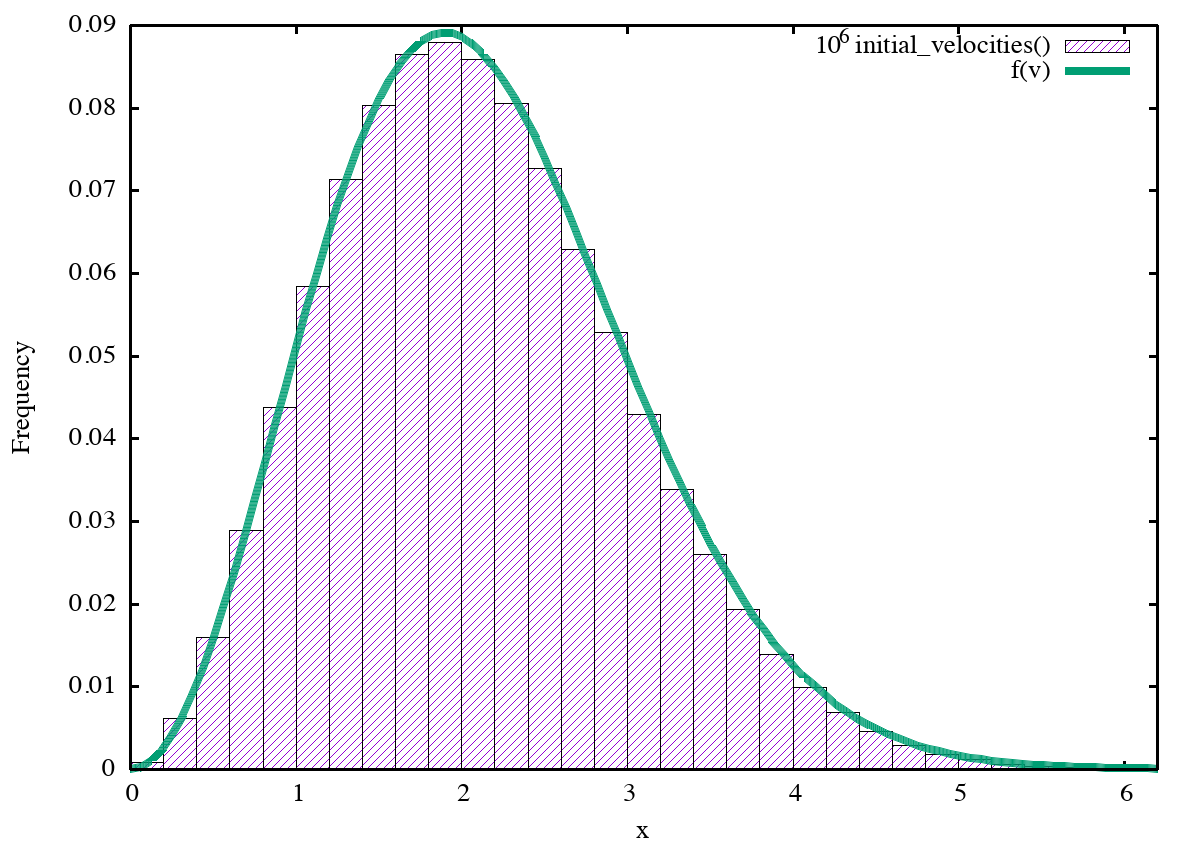
\includegraphics[width=0.5\textwidth]{Boltz.png}}
    \caption{Comparison between the geerated and expected gaussian distribution with $\mu=0,\sigma=1$}(a), and the velocity boltzamnn distribution with $\frac{K_bT}{m}=1$ (b).
    \label{fig:dist}
\end{figure}

\begin{lstlisting}[caption=Velocity initalization]
subroutine initial_velocities(velocities,nbr_atomes,temp,mass)
  implicit none

  real*8, dimension (:,:),intent(inout) :: velocities 
  real*8, intent(in) :: temp,mass
  integer, intent(in) :: nbr_atomes
  real*8 :: kb=3.166811d-6
  integer :: i,j

  do i=1,nbr_atomes
    do j=1,3
      velocities(i,j)=sqrt(kb*temp/mass)*gaussian_distr() ! Initial velocities following the Boltzmann distribution
    enddo
  enddo
end subroutine initial_velocities \end{lstlisting}

\section{Periodic boundary conditions}

To implement periodic boundry conditions (PBC) the subroutine \textit{get\_distances\_forces\_PBC} is added to the program. The subroutine takes as inputs the number of atoms, the positions, distances, forces, the box size (which has to be passed as an argument when calling the program), and $\sigma$ and $\epsilon$ of the Lennard-Jones potential. The distances and forces are updated for each atom.\\
\par
The subroutine calculates the distances and the forces using the nearest image of each particle pair. This translate that each unique particle only interacts once with each other unique particles (and not with itself). The downside of this approach is that the code will not be able to model a system with a small number of particles, like the provided example input of 10 Ar atoms. Arguably, PBC with such small systems are going to be unreallistic in any case. The subsequent calculations are performed with a bigger system of 125 Ar atoms.\\
Additionally, for better visualization, the atoms are constantly wrapped to the unit cell and, finally, this functionality is not allowed to be used with the SCP.\\

To test the performance of subroutine, the results from \cite{rahman1964correlations} are reproduced and compared. The radial distribution function is calculated for liquid argon at 94.4 K, $\epsilon=0.24$ K and $\sigma=3.4$ Å. The simulation is run with 125 particles (in \cite{rahman1964correlations} they use 864 particles) in a cubic box with periodic boundary conditions of 18.2 Å:

\begin{lstlisting}[language=bash]
    ./md_program -FILE liquid-argon.xyz -TIMESTEP 1 -PBC 18.206778313424067 -SAVEFREQ 100 -MAX_MD_STEPS 10000 -THERMO BEREN 2 -TEMP 94.4 -EPS 0.23846451108000002 -SIGMA 3.4 \end{lstlisting}

The trajectory is then analyzed using VMD to obtain the radial distribution function. It contains three peaks at 3.7 Å (g(r) = 3), 7.1 Å (g(r)=1.2) and 10.2 Å (g(r)=1.1) which are in agreement with the results of \cite{rahman1964correlations}.

\begin{figure}[h]
  \centering
  \subfloat[\textit{E(t)}]{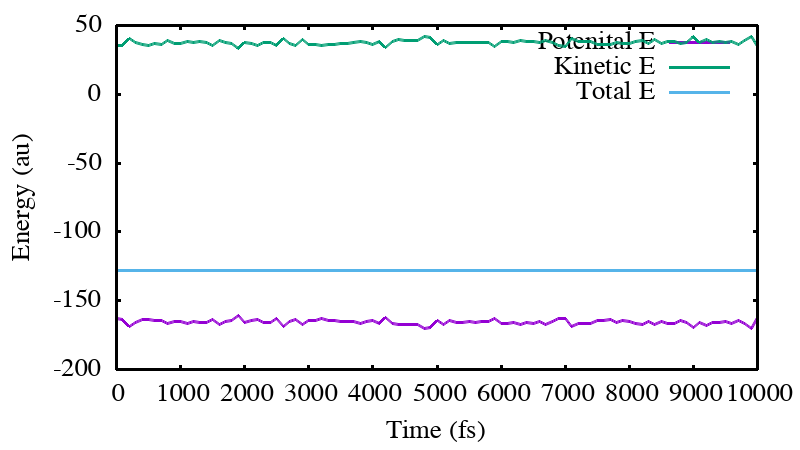
\includegraphics[width=0.5\textwidth]{PBC_E.png}}
  \subfloat[\textit{g(r)}]{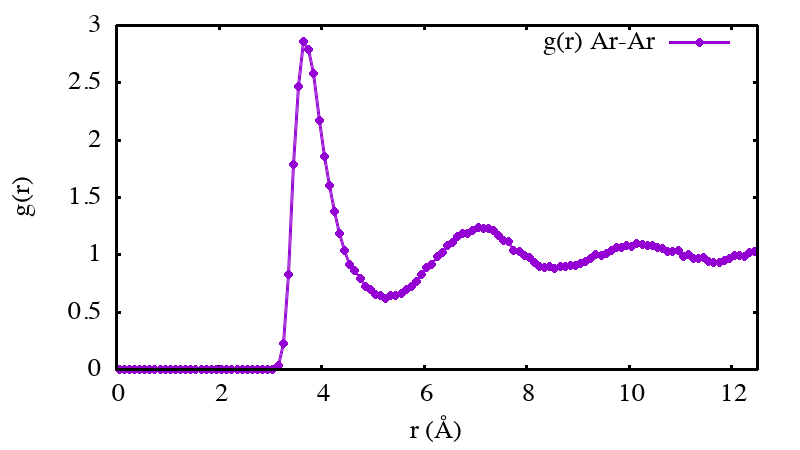
\includegraphics[width=0.5\textwidth]{Gr.png}}
  \caption{Left, energy evolution of the PBC simmulation. Right, radial distribution function for liquid argon at same conditions as in \cite{rahman1964correlations}.}
  \label{fig:PBC}
\end{figure}

\begin{figure}[h]
  \centering
  \subfloat[\textit{(1,1,1) box}]{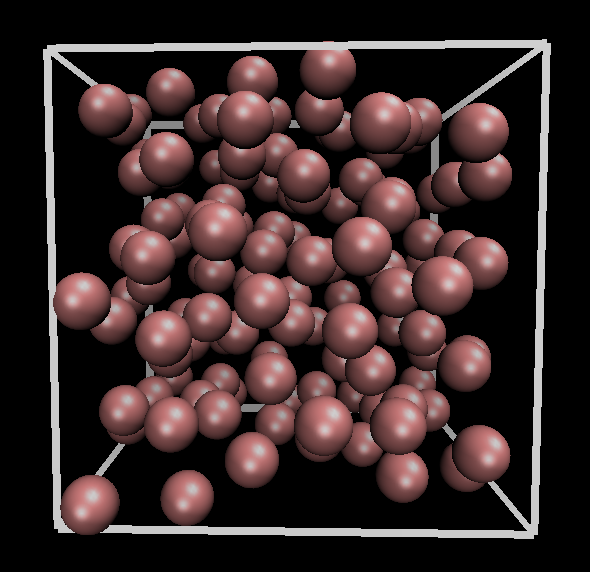
\includegraphics[height=0.35\textwidth]{PBC_111.png}}
  \hspace{1.5cm}
  \subfloat[(3,3,1) box]
  {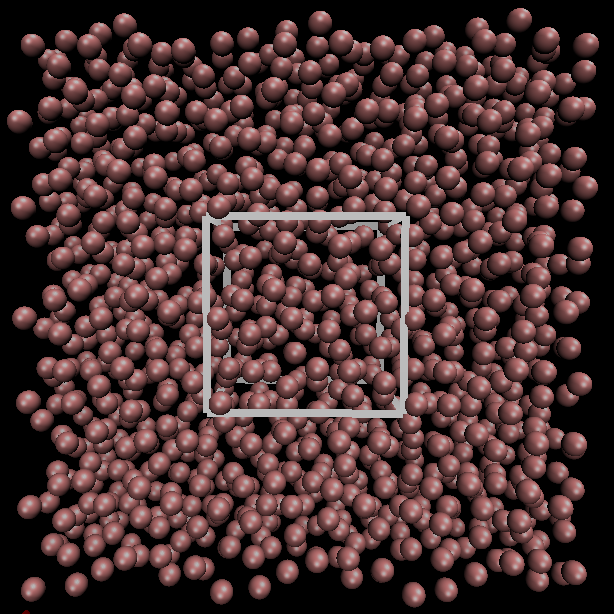
\includegraphics[height=0.35\textwidth]{PBC_331.png}}
  \caption{Snapshots of the PBC calculation. Left, unit cell ((1,1,1) box). Right, (3,3,1) superbox showing the system continuity. The unit cell is shown with white lines.}
  \label{fig:boxes}
\end{figure}

\begin{lstlisting}[caption=Subroutine to apply a PBC.]
    subroutine get_distances_forces_PBC(positions,distances,forces,nbr_atomes,L,sigma,eps)

    implicit none
    
    real*8, allocatable, dimension (:,:),intent(inout) :: positions
    real*8, allocatable, dimension (:,:),intent(inout) :: distances
    real*8, allocatable, dimension (:,:),intent(inout) :: forces
    
    real*8, intent(in)   :: L, sigma, eps
    integer, intent(in)  :: nbr_atomes
    
    real*8             :: dist
    real*8             :: sigma_12,sigma_6
    real*8             :: dist2
    real*8             :: dr4,dr8,dr14
    real*8             :: part_6,part_12
    integer            :: i,j,k
    
    forces=0.0d0
    distances=0.0d0
    
    do i=1,nbr_atomes-1 !calculate distances**2
      do j=i+1,nbr_atomes
        do k=1,3
          dist = positions(i,k)-positions(j,k)
          distances(i,j)=distances(i,j) + (dist - L*dble(nint(dist/L)))**2 !We use the nearest image of each particle pair
        enddo 
       distances(j,i)=distances(i,j)
      enddo
    enddo
    
    sigma_6=sigma**6*6.0d0 !calculate forces
    sigma_12=sigma**12*6.0d0
    
    do i=1,nbr_atomes-1
      do k=i+1,nbr_atomes
        do j=1,3
          dist2=positions(i,j)-positions(k,j) ! Need dist component for the F direction
          dist2=dist2-L*dble(nint(dist2/L)) ! closest image for PBC
          dr4=distances(i,k)*distances(i,k)
          dr8=dr4*dr4
          dr14=dr8*dr4*distances(i,k)
          part_6  = sigma_6*(-(dist2)/dr8)
          part_12 = sigma_12*(-(2.0d0*dist2)/dr14) 
          forces(i,j)=forces(i,j)-4.0d0*eps*(part_12-part_6)
          forces(k,j)=forces(k,j)+4.0d0*eps*(part_12-part_6)
        enddo
      enddo
    enddo
    endsubroutine get_distances_forces_PBC\end{lstlisting}

\begin{lstlisting}[caption=Forbid using SCP together with PBC.]
if (pbc .eqv. .TRUE.) then  !Apply PBC if activated
  call get_distances_forces_PBC(positions,distances,forces,nbr_atomes,Box_L,sigma,eps)
else
  call get_distances(positions,distances,nbr_atomes)
  call get_forces(forces,distances,positions,nbr_atomes,sigma,eps)
  if (scp .eqv. .TRUE.) then ! Apply SCP if activated
    call apply_scp(forces,energy_pot,positions,nbr_atomes,R_scp)
  endif
endif \end{lstlisting}

\printbibliography
\end{document}

